\documentclass[../../main]{subfiles}

\renewcommand\thesection{\arabic{section}}


\begin{document}

\section{Buffer / Inverter} \label{sec:}

The custom boards we will be designing in the coming chapters will require \emph{buffers}
here and there in order to strengthen signals, so this section introduces a simple
RTL\footnote{Resister Transistor Logic} buffer. Additionally, these \emph{boards} require
some other \emph{logic gates} too. One among them is an \emph{inverter}.

If we want to design an RTL buffer, we could simply \emph{cascade} two inverters. But we
could save one inverter, if we choose to use an \emph{inverter} as a \emph{buffer} at
the cost of \emph{flipping} the logic.

\alertNote{
    Since we are using an \emph{inverter} as a \emph{buffer}, the input logic to the
    \emph{buffer} also \emph{inverts}. If we want the output to be \emph{high} then
    the input to the buffer should be \emph{low}, so the rest of the circuit is needed to
    be designed accordingly with this change in mind.
}

We have some design requirements. These inverts / buffers are either driven by
\textbf{74LS}\footnote{They are TTL based.} ICs or \esp. \textbf{74LS} ICs are known
for their low $\si{V}_{OH}$ and low source current. Logic high of \textbf{74LS} series ranges
from $2.2\si{V}$ to $3\si{V}$. And can only source upto $0.4\si{mA}$. So we need to
design an inverter with this in mind.

We need to choose a BJT that can be driven with a small input current. \emph{BC547} is
good candidate for our scenario. Refer Figure \ref{fig:bc547Pinout} for pinout and Table
\ref{tbl:bc547Spec} for a brief specification of \emph{BC547}.

{\begin{minipage}[c] {0.42\textwidth}
    \centering
    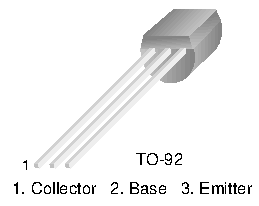
\includegraphics [
    ] {pics/bc547.pdf}
    \captionof{figure} {
        Pinout of \textbf{BC547}.
        \label{fig:bc547Pinout}
    }
\end{minipage}
\begin{minipage}[c] {0.52\textwidth}

    \begin{tabularx} {\linewidth} {
            *{1}{>{\centering\arraybackslash}m{0.5\linewidth}}
            *{1}{>{\centering\arraybackslash}m{0.5\linewidth}}
        }
        \toprule
        Parameter & Value \\
        \midrule
        $\si{V}_{CEO}$ Max. & $45 \si{V}$ \\
        $\si{V}_{EBO}$ Max. & $6 \si{V}$ \\
        $\si{I}_{C}$ Max. & $100 \si{mA}$ \\
        $\si{P}_{C}$ Max. & $500 \si{mW}$ \\
        $\si{C}_{ob}$ (Output Capacitance) Max. & $6 \si{pF}$ \\
        \bottomrule
    \end{tabularx}
    \captionof{table} {
        Brief specification of \textbf{BC547}.
        \label{tbl:bc547Spec}
    }
\end{minipage}}

\end{document}
